\documentclass{article}
\usepackage{enumerate}
\usepackage{enumitem}
\usepackage[utf8]{inputenc}
\usepackage{latexsym,amsfonts,amssymb,amsthm,amsmath}
\usepackage{graphicx}
\usepackage{caption}
\usepackage{float}
\usepackage{bbm}
\usepackage{tcolorbox}
\usepackage{indentfirst}
\usepackage[colorlinks=true]{hyperref}
\title{Indian Institute of Technology Delhi\\COL774: Machine Learning\\Fall 2024-2025\\Practice Problems}
\author{Harshit Goyal}
\date{November 2024}
\usepackage[a4paper, left=1.0in, right=1.0in]{geometry}

\newcommand*{\xieg}{\mathbf{x}^{(i)}}
\newcommand*{\xupi}{x^{(i)}}
\newcommand*{\xhati}{\hat{\mathbf{x}}^{(i)}}
\newcommand*{\yieg}{y^{(i)}}
\newcommand*{\zieg}{z^{(i)}}
\newcommand*{\yhatieg}{\hat{y}^{(i)}}
\newcommand*{\loss}{\mathcal{L}}
\newcommand*{\data}{\mathcal{D}}
\newcommand*{\wb}{\mathbf{w}}
\newcommand*{\mM}{\mathbf{M}}
\newcommand{\gdaparm}{\phi, \boldsymbol{\mu}_0, \boldsymbol{\mu}_1, \boldsymbol{\Sigma}_0, \boldsymbol{\Sigma}_1}
\newcommand*{\re}{\mathcal{R}}
\newcommand*{\bsigma}{\boldsymbol{\Sigma}}
\newcommand*{\bmu}{\boldsymbol{\mu}}
\newcommand*{\mv}{\mathbf{v}}
\newcommand*{\me}{\mathbf{e}}

\newcommand*{\bphi}{\boldsymbol{\phi}}

\newcommand*{\bu}{\mathbf{u}}
\newcommand*{\bz}{\mathbf{0}}
\newcommand*{\mz}{\mathbf{z}}
\newcommand*{\mZ}{\mathbf{Z}}
\newcommand*{\mA}{\mathbf{A}}
\newcommand*{\mE}{\mathbf{E}}
\newcommand*{\malpha}{\boldsymbol{\alpha}}
\newcommand*{\mc}{\mathbf{C}}
\newcommand*{\mb}{\mathbf{b}}
\newcommand*{\mx}{\mathbf{x}}
\newcommand*{\md}{\mathbf{d}}
\newcommand*{\expect}{\mathbb{E}}
\newcommand*{\my}{\mathbf{y}}
\newcommand*{\mQ}{\mathbf{Q}}
\newcommand*{\mX}{\mathbf{X}}
\newcommand*{\mC}{\mathbf{C}}
\newcommand*{\mY}{\mathbf{Y}}
\newcommand*{\mf}{\mathbf{f}}
\newcommand*{\mt}{\mathbf{t}}
\newcommand*{\mmu}{\mathbf{u}}
\newcommand*{\bU}{\mathbf{U}}
\newcommand*{\beps}{\boldsymbol{\epsilon}}

\newcommand{\norm}[1]{\left\lVert#1\right\rVert}
\newcommand{\maxbelow}[1]{\max\limits_{#1}}
\newcommand{\minbelow}[1]{\min\limits_{#1}}

\newcommand{\at}[2][]{#1|_{#2}}
\DeclareMathOperator*{\argmax}{arg\,max}
\DeclareMathOperator*{\argmin}{arg\,min}


\begin{document}

\maketitle

\section{About}
The most recent version of this document can be found on the \href{https://github.com/Harshit0143/COL774-Machine-Learning-Fall-2024-2025.git}{project repository}. We encourage you to use this work further. Please see the \href{https://github.com/Harshit0143/COL774-Machine-Learning-Fall-2024-2025.git}{project repository} for the BiBTex citation.\\\\
This problem set was written by me, \href{https://github.com/Harshit0143/}{Harshit Goyal} during the Teaching Assistantship for the COL774 Fall Machine Learning course 2024-2025, offered by \href{https://www.cse.iitd.ac.in/~rahulgarg/}{Prof Rahul Garg}. We thank the students in this class for feedback on many of these problems.

\tableofcontents
\section{Introduction}\label{intro}
\begin{enumerate}
\item 
You may refer to \cite{Petersen2012} for matrix derivatives for the upcoming problems.
\item Below notations are consistent throughout the document.
\item The dataset is denoted as $\data = \{(\xieg, \yieg)\}_{i = 1}^{m}$ where $\xieg \in \re^{n}$ and $\yieg \in \re^{n}$ for Linear Regression. Further $\yieg \in \{0, 1\}$ for Logistic Regression.
\item $\wb \in \re^n$ and $\wb = \left[ \begin{smallmatrix} w_1 & w_2 & w_3 & \dots & w_n \end{smallmatrix} \right]^T$.
\item For Linear Regression,  $\yhatieg =  \wb^T \xieg + b$.
\item For Logistic Regression,  $\yhatieg =  g(\wb^T \xieg + b)$, where $g: \re \to \re$ is an activation function.
\item  \label{loss_functions}
\begin{align*}
\loss_{SSE}(\wb, b) &= \frac{1}{m}\sum_{i = 1}^{m}(\yieg - \yhatieg)^2\\
\loss_{Logistic}(\wb, b) &= -\frac{1}{m}\sum_{i = 1}^{m} \yieg\log(\yhatieg) + (1 - \yieg)\log(1 - \yhatieg)\\ 
\loss_2(\wb,b) &= \wb^T\wb\\
\loss_1(\wb,b) &= \sum_{i = 1}^{n} |w_i|\\
\end{align*}

\item When the bias term is taken as a feature, the absorb $b$ in $\wb$ and the loss functions in \autoref{loss_functions} can be denoted as $\loss_{SSE}(\wb)$, $\loss_{Logistic}(\wb)$, $\loss_2(\wb)$, $\loss_1(\wb)$, respectively.
\end{enumerate}
\newpage
\section{Regression}
\subsection{GFLOPS Calculation}



For matrix multiplication \( \mathbf{Y} = \mathbf{WX} \), where \( \mathbf{X} \in \re^{m \times n}\)  matrix and \( \mathbf{W} \in \re^{n \times 1}\):

\begin{enumerate}
    \item \textbf{Using a Python implementation with nested for loops:}
    \begin{itemize}
        \item Calculate the GFLOPS (Giga-Floating Point Operations Per Second) for the matrix multiplication operation. Determine the total number of floating-point operations involved, including both multiplication and addition operations, divide this by the time taken to execute the matrix multiplication, and convert the result to GFLOPS by dividing by \( 10^9 \).
    \end{itemize}

    \item \textbf{Using Python’s \texttt{numpy} library:}
    \begin{itemize}
        \item Similarly, calculate the GFLOPS for the matrix multiplication operation using \texttt{numpy}'s built-in matrix multiplication function.
    \end{itemize}

    \item \textbf{Comparison and Visualization:}
    \begin{itemize}
        \item Plot a graph with the x-axis representing \(m\) (considering constant \(n\)) and the y-axis representing GFLOPS to illustrate the performance difference between the two implementations.
    \end{itemize}
\end{enumerate}



\subsection{Binary Classification}


For binary classification using the sigmoid function, write the gradient descent update rule for the following methods:

\begin{enumerate}
    \item \textbf{Stochastic Gradient Descent (SGD):} \\
    Update the model parameters using one data point at a time.

    \item \textbf{Batch Gradient Descent:} \\
    Update the model parameters using the entire dataset.

    \item \textbf{Mini-Batch Gradient Descent:} \\
    Update the model parameters using a subset of the dataset (a mini-batch).
\end{enumerate}

Use the sigmoid function \( \sigma(z) = \frac{1}{1 + e^{-z}} \).

\subsection{GDA classification and GMM clustering}
We have $\data = \{(\xieg, \yieg)\}_{i = 1}^{m}$ where $\xieg \in \re^n$ and $\yieg \in \{1, 2, \dots, k\}$. $\data$ was generated by first selecting $\yieg$ in $\{1, 2, \dots, k\}$ using $\text{Multinoulli}(\bphi)$, $\phi \in \re^{k}$, and then choosing $\xieg$ from $\mathcal{N}(\bmu_j, \bsigma_j), \bmu_j \in \re^n, \bsigma \in \re^{n \times n}, j \in \{1, 2, \dots, k\}$, where $j$ is the label picked earlier. This process is independent for each example.\\

When the labels $\yieg$ are hidden (not available to us), they are denoted as $\zieg$ and we can run the GMM algorithm on the data to figure out which examples belong to which "cluster" (and not class as that is unknown).

\begin{enumerate}[label=\alph*)]
\item Set up the MLE problem, and give MLE estimates for parameters $\bphi, \bmu_j, \bsigma_j$. Do this by maximizing $p(\{(\xieg, \yieg)\}_{i = 1}^{m})$. Recall our discussion from \nameref{sec:gda}.
\item Now, let us say in the data $\data$, for very few examples, the labels $\yieg$ are missing. How will you label these examples for another downstream task that needs to be labeled $\data$.
\end{enumerate}


\subsection{Modified GMM Clustering}
We have data $\data = \{\xieg\}_{i = 1}^{m}, \xieg \in \re^n$. Consider clustering using GMM. We modify it slightly here. We now model,
\begin{align*}
    \zieg &\sim \text{Multinoulli}(\bphi)\\
    \xieg \ \ | \ \ (\zieg = j) &\sim \mathcal{N}(\bmu_j, \sigma^2 \mathbf{I}_n) \quad j \in \{1, 2, \dots, k\}
\end{align*}
Here $\bphi \in \re^k, \bmu_j \in \re^n$ are learnable but $\sigma^2 > 0$ is a \textbf{hyperparameter}.
\begin{enumerate}[label=\alph*)]
\item Write down \textbf{E. Step} (update of $w_{ij}$) and \textbf{M. Step} (update of learnable parameters) for this problem.

\item Using $w_{ij}$ computed in the above problem, show that in the limit $\sigma \to 0^{+}$, the algorithm becomes the K-means  clustering algorithm.
\end{enumerate}
\subsection{Probabilistic Interpretation of Regularization}

In class we looked at the Maximum Likelihood Estimate of $\wb$ for the Linear Regression problem. We considered $\wb$ as parameter and the optimum $\wb_{MLE}$ (for a single example) was defined as
$$\wb_{MLE} = \argmax_{\wb} P(\yieg | \xieg ; \wb)$$

Now, let's treat $\wb$ as a Random Variable, distributed as (this is called a \textbf{priori} on $\wb$)
$$\wb \sim  \mathcal {N}(\mathbf{0},\mathbf{\Sigma})$$
where $\mathbf{\Sigma} = diag\{\lambda_1, \lambda_2..\lambda_n\}$ and $\lambda_1, \lambda_2.....\lambda_n > 0$. We now define $\wb_{MAP}$ (MAP stands for \textbf{M}aximum \textbf{a} \textbf{P}osteriori) as 

\begin{equation}\label{w_MAP}
\wb_{MAP} = \argmax_{\wb} P(\yieg | \xieg, \wb) P(\wb)
\end{equation}
Now, similar to the MLE case, we assume, over all examples, $\yieg - \yhatieg| \xieg, \wb$ are $i.i.d$ distributed as
\begin{equation*}
\yieg - \yhatieg| \xieg, \wb \sim \mathcal{N}(0, \sigma^2)
\end{equation*}

\begin{enumerate}[label=\alph*)]
\item 
Simplify \autoref{w_MAP} for the entire dataset combined now, and show solving $\wb_{MAP}$ is similar to Linear Regression with $L_2$ Regularization on $\wb$.
\item 
Obtain explicitly, the \textbf{priori} on $\wb$ that will lead to the $L_1$ Regularization of $\wb$ (keep different penalty coefficient for each of the $n$ components of $\wb$). Does this distribution have a name?\\

Solution to above part. It's called the \textbf{Laplace Distribution}.
    $$p(w_1, w_2...w_n) = \prod_{i=1}^{n}\frac{\lambda_i}{2}e^{-\lambda_i |w_i|}$$
\end{enumerate}






\subsection{Logistic Regression in Perfectly Linearly Separable case}

\begin{figure}[H]
    \centering
    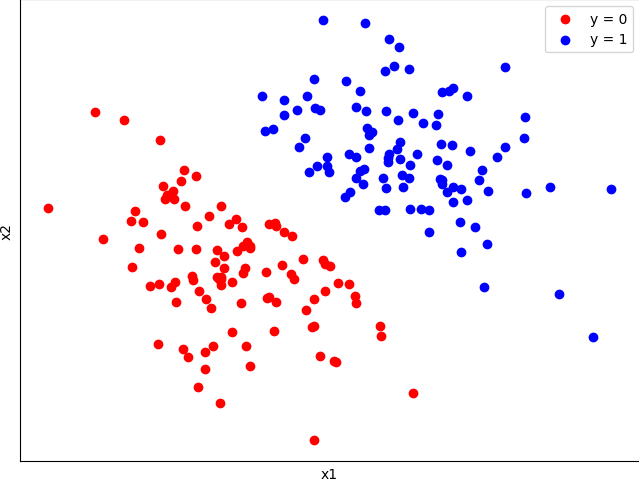
\includegraphics[width=0.5\textwidth]{images/gaussian_separable_data_plot.png}
    \caption{Data for Logistic Regression, features $x_1$ and $x_2$}
    \label{fig:linearly_separable}
\end{figure}

Consider Logistic Regression on \textbf{Perfectly Linearly Separable} data, as shown in \autoref{fig:linearly_separable}. You may not assume that there are just $2$ features as shown in the figure.

\begin{enumerate}[label=\alph*)]
\item What is the condition (possibly implicit) for a data to be linearly separable, when the features $\xieg \in \re^n$.

\item Consider solving for the decision boundary $(\wb, b)$ for such data. Show what $\forall \epsilon > 0 \ \ \exists (\wb_{\epsilon}, b_{\epsilon})$ such that $\loss_{Losgistic}(\wb, b) < \epsilon$.

\item Consider running gradient descent, to obtain $(\wb, b)$. Assuming the learning rate is small, will the algorithm ever converge in $(\wb, b)$? (Answer: $\wb$ and $b$ diverge. You may skip it as it's difficult to prove.)
\end{enumerate}





\subsection{Logistic Regression for multiple classes}

Consider $r$ class classification problem. We build a model that predicted an input belonging to each of the $r$ classes (similar to Logistic Regression).

The model is parametrized by $r$ weight vectors, $\wb_1, \wb_2...\wb_r$. For an input $\xieg$, the model is evaluated as,

\begin{align}
z_j^{(i)} = \wb_j^T \xieg \ \ \text{ for j } = 1,2 ....r\\
\hat{y}^{(i)}_j = \frac{e^{z_j}}{\sum_{k = 1}^{r} e^{z_k}} \ \ \text{ for j } = 1,2 ....r\label{softmax}
\end{align}

\autoref{softmax} is the Softmax function. (Why \textbf{Soft}max?) The loss function, for a single example $(i)$, $\yieg \in \{1,2....r\}$ is
\begin{equation}\label{cross_entropy}
    \loss^{(i)}(\wb_1, \wb_2...\wb_r) = -\sum_{j = 1}^{r} \mathbbm{1}_{\{\yieg = j\}} \log(\yhatieg_j)
\end{equation}

Where $\mathbbm{1}_{(.)}$ is the indicator function.
\[
\mathbbm{1}_{(x)} = 
\begin{cases} 
1 & \text{if } x \text{ is True} \\
0 & \text{if } x \text{ is False}
\end{cases}
\]

\autoref{cross_entropy} is know is the \textbf{Cross Entropy Loss function}. Now, define 
$$\loss(\wb_1, \wb_2...\wb_r) = \sum_{i = 1}^{m} \loss^{(i)}(\wb_1, \wb_2...\wb_r)$$

\begin{enumerate}[label=\alph*)]
\item  Is $\loss(\wb_1, \wb_2...\wb_r)$ convex? (Answer: Yes! But you may skip it as the proof gets very involved.)
\item Obtain explicitly, $\nabla_{\wb_1} \loss, \nabla_{\wb_2} \loss.....\nabla_{\wb_r} \loss$. Hint: Start by writing $\loss$ in terms of $(\wb_1, \wb_2...\wb_r)$.
\end{enumerate}

\subsection{LASSO for feature selection}

\cite{Goodfellow-et-al-2016} have mentioned in the chapter \textbf{Regularization for Deep Learning}, 
\begin{center}
     \textit{"the well known LASSO (Tibshirani, 1995) (least absolute shrinkage and selection operator) model integrates an $L_1$ penalty with a linear model and a least-squares cost function. The $L_1$ penalty causes a subset of the weights to become zero, suggesting that the corresponding features may safely be discarded."}
\end{center}


We'll see in this problem how. Let $x \in \re$. Let $a > 0, \lambda > 0, b, c, x \in \re$ and 

\begin{align*}
w^* &=\argmin_{x} ax^2 + bx + c\\
w(\alpha) &= \argmin_{x} ax^2 + bx + c + \alpha |x|\\
\end{align*}

\begin{enumerate}[label=\alph*)]
\item Compute $w(\alpha)$ in terms of $\alpha, a, w^*$. What do you conclude?

\item Now let's consider multiple features. Let $\mA = diag(a_1, a_2\hdots, a_n), a_i > 0 \ \ \forall i$ and $\mb \in \re^n$. 
\begin{align*}
    \wb^* &= \argmin_{\mx \in \re^n} \mx^T \mA \mx + \mb^T \mx + c\\
    \wb(\alpha) &= \argmin_{\mx \in \re^n} \mx^T \mA \mx + \mb^T \mx + c + \alpha\norm{\mx}_1\\   
\end{align*}
Show that 
\begin{equation*}
    \wb(\alpha)_i = sign(\wb_i)\max(0, |w_i| - \frac{\alpha}{a_i})
\end{equation*}
What happens to components of $\wb(\alpha)$ corresponding to smaller diagonal entries of $\mA$? How can this be used for feature selection?
\end{enumerate}




\subsection{Limit of Locally Weighted Linear Regression}
The problem idea was suggested to me by \href{https://www.cse.iitd.ac.in/~rahulgarg/}{Prof. Rahul Garg}. Recall Locally Weighted Linear Regression done in class. We'll understand what happens in the limit, hyper-parameter $\sigma \to \infty$ and $\sigma \to 0^+$. 
Consider points $x_1 <  x_2 < x_3....x_m \in \re$ and $\lambda > 0$ be fixed. We need to regress over points $(x_1, y_1), (x_2, y_2) \hdots (x_m, y_m)$. 
The loss function, for a point $x \in \re$ is

\begin{align*}
\alpha_{\sigma, i}(x) &= \frac{e^{-\frac{(x - x_i)^2}{2\sigma^2}}}{\sum_{j = 1}^{m} e^{-\frac{(x - x_j)^2}{2\sigma^2}}}\\
\hat{y}_i &= w x_i + b\\
\loss_{\sigma}(x, w, b) &= \frac{1}{m}\sum_{i = 1}^{m} \alpha_{\sigma, i}(x)(y_i - \hat{y}_i)^2 + \lambda w^2
\end{align*}

Denote \begin{align*}
w_{\sigma}(x), b_{\sigma}(x) &= \argmin_{w, b}\loss_{\sigma}(x, w, b)\\
f_{\sigma}(x) &= w_{\sigma}(x) x + b_{\sigma}(x)
\end{align*}

\begin{enumerate}[label=\alph*)]
\item Obtain $f_{\infty}(x) = \lim_{\sigma \to \infty} f_{\sigma}(x)$.
\item Obtain $f_{0}(x) = \lim_{\sigma \to 0^{+}} f_{\sigma}(x)$.
\end{enumerate}



\subsection{Unique Minima}\label{prob:unique_minima}
In class we discussed that the problem of Linear Regression has a unique optimum. We'll try to prove that formally and see what happens to stationary points when convexity is not guaranteed. Consider the function

\begin{equation}\label{unique_minima_objective}
\mf(\mx) = \frac{1}{2} \mx^T \mA \mx - \mb^   T\mx + c 
\end{equation}
Where $c\in \re, \ \  \mx  \in \re^n, \ \ \mb \in \re^n, \ \ \mA \in \re^{n \times n}$ and is Symmetric. All eigenvalues of $\mA$ are positive. We define $\mx^* \in \re^n$ such that $\nabla_\mx f |_{\mx = \mx ^ *} = 0$.

\begin{enumerate}[label=\alph*)]
\item Show that $\mA$ is invertible and hence $\mx^*$ exists uniquely.
\begin{equation} \label{p2_minima}
    \mf(\mx) - \mf(\mx^*) > 0 \ \ \forall \mx \in \re^n  -  \{\mx^*\}
\end{equation}
\item  We'll now prove \autoref{p2_minima}. Set $\mx = \mx^* + \epsilon \mz$, $\mz^T\mz = 1$, $\epsilon > 0$  in the equation, and show that
\begin{equation}
      \mf(\mx^* + \epsilon\mz) - \mf(\mx^*) = \frac{\epsilon^2}{2}\mz^T\mA \mz
\end{equation}

Assume the fact, "Every $n \times n$ Real Symmetric Matrix is Diagonalizable and has a set of $n$ Orthonormal Eigenvectors". Express $\mz$ as
\begin{equation*}
    \mz = \sum_{i = 1}^{n} a_i \mv_i
\end{equation*}
Where $\mv_i^T\mv_i = \delta_{ij}$ and $\lambda_i$ be the Eigenvalue of $\mA$ corresponding to $\mv_i$. Show that
\begin{equation}
      \mf(\mx^* + \epsilon\mz) - \mf(\mx^*) = \frac{\epsilon^2}{2}\sum_{i = 1}^{n} a_i^2 \lambda_i
\end{equation}


\item Now, let all eigenvalues of $\mA$ be non-zero and not all of the same sign. Obtain \textbf{explicitly}, atleast one $\mz \in \re^n$ such that  $\norm{z}_2 = 1$ and $\mf(\mx^* + \epsilon \mz) - \mf(\mx^*) < 0$ for some $\epsilon > 0$.

\item Show that the Linear Regression objective can be expressed \autoref{unique_minima_objective}. Does the condition, "$\mA$ is Symmetric. All eigenvalues of $\mA$ are positive" assumed here always hold in linear Regression? Clearly describe the condition on the data when this isn't true. We'll derive these conditions in \nameref{prob:dependent_factors}.
\end{enumerate}

% \subsubsection*{Hint}
% \begin{enumerate}
%     \item \label{p2_hint_1} In  \autoref{p2_minima}, parametrize $\mx$ as $\mx = \mx^* + \epsilon\mt$ where $\epsilon \in \re, \ \ \mt \in \re^n$ and  $\norm{t}_2 = 1$. It solves to $\mf(\mx) - \mf(\mx^*) = \frac{\epsilon^2}{2} \mt^T \mA \mt > 0 \ \ \forall$ directions $\mt$.

% \item Express $\mt$ as a linear combination of the eigenvectors of $\mA$. You'll need to use the facts "Every Real Symmetric Matrix is diagonalisable" and "For a Real Symmetric Matrix, Eigenvectors corresponding to distinct eigenvalues are Orthogonal". 
% \item If $(\mmu_1, \mmu_2...\mmu_n)$ are normalized eigenvectors of $\mA$ (chosen orthogonal\footnote{$\mA$ is Symmetric, so eigenvectors corresponding to distinct eigenvalues are orthogonal. If eigenvalues are repeated, you can choose an orthogonal basis for the that eigenspace.}) with eigenvalues $(\lambda_1, \lambda_2...\lambda_n)$. Let 
% $\mt = \sum_{i = 1}^{n} a_i \mmu_i$ with $\sum_{i = 1}^{n} a_i^2 = 1$ then 
% \begin{equation*}
%  \mf(\mx) - \mf(\mx^*) = \frac{\epsilon^2}{2}\sum_{i = 1}^{n} a_i^2 \lambda_i
% \end{equation*}
% Choose $a_i = 1$ such that $\lambda_i < 0$ to solve c). Similarly you can see the change in $\mf(\mx)$ on moving in any direction.

% \end{enumerate}

\subsection{Multiple Minimas}\label{prob:dependent_factors}
In this problem we'll re what happens when $\mA$ in \nameref{prob:unique_minima} has some eigenvalues $0$. Consider the data matrices, $\mX \in \re^{m \times n}$ and $\mY \in \re^{m}$.
\begin{equation*}
\mX =    
\begin{pmatrix}
\mathbf{x}^{(1)T}\\
\mathbf{x}^{(2)T}\\
\vdots \\
\mathbf{x}^{(m)T}\\
\end{pmatrix}
\ \ 
\mY=    
\begin{pmatrix}
y^{(1)}\\
y^{(2)}\\
\vdots \\
y^{(m)}\\
\end{pmatrix}
\end{equation*}

Absorb the bias term in Linear Regression into $\xieg$'s. We derived the condition for the optimal $\wb^{*}$ as (derive it yourself if you don't remember this),
\begin{equation}\label{equation:minima_condition}
    \mX^T\mX\wb^* = \mX^Ty
\end{equation}

When $\mX^T\mX$ is invertible, we get
\begin{equation}
    \wb^* = (\mX^T\mX)^{-1}\mX^Ty
\end{equation}

We'll now examine precisely when is $\mX^T\mX$ not invertible.

\begin{enumerate}[label=\alph*)]
\item Show that \autoref{equation:minima_condition} has atleast one solution.
\item Show that all $\wb^*$ satisfying \autoref{equation:minima_condition} lead to the same $\loss_{SSE}(\wb^*)$ value.
\item 
Show that a square matrix $\mA \in \re^{n \times n}$ is not invertible if and only if $\mA \mv = \mathbf{0}$ for some non-zero $\mv \in \re^n$.

\item For any $\mv \in \re^n$, show that \begin{equation}
 \mX^T\mX\mv = \bz \iff \mX\mv = \bz   
\end{equation} 
If you need a hint, see this\footnote{For $\mz 
\in \re^n$, $\mz^T\mz = 0 \iff \mz = \bz$.}. If you're up for a challenge (this will not be used in later parts), let $\mC \in \re^{m \times m}$ be a fixed, Symmetric Positive Definite matrix, show that 
\begin{equation*}
\mX^T\mC\mX\mv = \bz \iff \mX\mv = \bz
\end{equation*}


\item  \label{dependent_factors_c}
Now let $\mX^T\mX$ be non-invertible. Using the above part, what do you conclude about the columns of $\mX$, the data matrix (note that there's also the column of all $1$'s in $\mX$). Let $\wb_1^*$ be one $\wb$ minimizing $\loss_{SSE}(\wb)$, obtain another.
% i.e. there $\exists \mv \in \re^n - \{\bz\}$ such that $\mX\mv = \bz$.
\item \label{dependent_factors_d}
Continuing \autoref{dependent_factors_c}, if you have to choose a subset of the initial $n$ features, for regression, without losing any information, how would you do that?

\item Following, the above part, can you realize why assuming $\mA$ in \nameref{prob:unique_minima} to be positive definite, instead of positive semi-definite, is reasonable and doesn't lead to loss of generality?

\item Redo all above parts for Weighted Linear Regression, with example-wise weights, $u_1, u_2...u_m$, all positive. You'll see all these results hold true for this case too! 
\end{enumerate}


\subsection{Is this Linear Regression?}
Consider this regression problem. Here $n > 4$ and the prediction
$$\yhatieg = \wb^T \xieg$$

We have $4$ \textbf{Linearly Independent Constraints} on $\wb$ represented as 
\begin{align*} \label{p1_constraints}
\mathbf{M}\wb = \mathbf{0}
\end{align*}
i.e. $\mathbf{M} \in \re^{4 \times n}$ and $rank(\mathbf{M}) = 4$.
Under the above constraints obtain the optimum value of $\mathbf{w}$ that minimizes these loss functions.


\begin{enumerate}[label=\alph*)]
  \item \begin{equation*}
   \loss_{SSE}(\wb)
\end{equation*}
  \item
 \begin{equation*}
   \loss_{SSE}(\wb) + \lambda \mathbf{w}^T \mA \mathbf{w}
\end{equation*}

Where $\lambda \in \mathcal{R}^{+}$ and $\mA$ is a \textbf{Symmetric Positive Definite Matrix}, are \textbf{constants}.
\end{enumerate}

Note that it is not intended that one uses Lagrangian Multipliers to solve this. 


% \subsubsection{Solution}

% Since $\mM$ has size $4 \times n$ and has rank $4$. It must have a sub-matrix of rank $4$. For simplicity, we'll assume the it's last $4$ rows and columns of $\mM$ (otherwise we can rename/ rearrange features to get this). Denote
% \begin{align*}    
% \mM &= \begin{bmatrix}
%     \mM_1 & \mM_2
% \end{bmatrix}\\
% \wb &= \begin{bmatrix}
%     \wb_1 \\
%     \wb_2
% \end{bmatrix}\\
% \mX &= \begin{bmatrix}
%     \mX_1 & \mX_2
% \end{bmatrix}
% \end{align*}

% Where $\mM_1$ and $\mM_2$ have sizes ${4 \times (n - 4)}$ and ${4 \times 4}$. $\wb_1$ and $\wb_2$ have sizes $(n - 4)$ and $4$. $\mX_1$ and $\mX_2$ have sizes ${m \times (n - 4)}$ and ${m \times 4}$ respectively. Note that $\mM_2$ is invertible. 

% Now, 
% \begin{align*}
% &\begin{bmatrix}
%     \mM_1 & \mM_2
% \end{bmatrix}
%  \begin{bmatrix}
%     \wb_1 \\
%     \wb_2
% \end{bmatrix} = \bz \\
% \implies &\mM_1 \wb_1 + \mM_2 \wb_2 = \bz\\
% \implies &\wb_2 = \mM_2^{-1}\mM_1 \wb_1
% \end{align*}
% Denote $\mZ = \mM_2^{-1}\mM_1$. We can see that,
% \begin{align*}
% \loss_{SSE}(\wb_1) &= (\mX\wb - \mY)^T(\mX\wb - \mY) \\
% &= (\begin{bmatrix}
%     \mX_1 & \mX_2
% \end{bmatrix} \begin{bmatrix}
%     \wb_1 \\
%     \mZ \wb_1
% \end{bmatrix} - \mY)^T(\begin{bmatrix}
%     \mX_1 & \mX_2
% \end{bmatrix} \begin{bmatrix}
%     \wb_1 \\
% \mZ \wb_1
% \end{bmatrix}\ - \mY) \\
%  &= ((\mX_1 + \mX_2 \mZ) \wb_1 - \mY)^T((\mX_1 + \mX_2 \mZ)\wb_1 - \mY)
% \end{align*}

% Denote $(\mX_1 + \mX_2 \mZ) = \mX_3$, and noting that $\wb_1$ is unconstrained it's easy to minimize

% \begin{equation*}
%      \loss_{SSE}(\wb_1)= (\mX_3 \wb_1 - \mY)^T(\mX_3\wb_1 - \mY)
% \end{equation*}



% \subsection*{Hints}
% \begin{enumerate}
%   \item You can reduce the problem to a standard Linear Regression Problem
%   \item The below matrix is $\mathbf{invertible}$, when $i,j,k,l$ are distinct as $\alpha_i$'s are pairwise distinct.

% \[
% C = \begin{bmatrix}
% 1 & 1 & 1 & 1 \\
% \alpha_i & \alpha_j &  \alpha_k & \alpha_l\\
% \alpha_i^2 & \alpha_j^2 &  \alpha_k^2 & \alpha_l^2\\
% \alpha_i^3 & \alpha_j^3 &  \alpha_k^3 & \alpha_l^3\\
% \end{bmatrix}
% \]
%   \item Set $(i,j,k,l)$ to $(k-3, k-2,k-1,k)$.
%   \item Obtain $\begin{bmatrix}
% w_{k - 3} & w_{k - 2} & w_{k - 1} & w_k
% \end{bmatrix}^T$ in terms of $\begin{bmatrix}
% w_{1} & w_{2} &  \cdots & w_{k - 4}
% \end{bmatrix}^T$ and optimize the latter vector.

% \end{enumerate}





\newpage
\section{Neural Networks}
\subsection{GDA classification and GMM clustering}
We have $\data = \{(\xieg, \yieg)\}_{i = 1}^{m}$ where $\xieg \in \re^n$ and $\yieg \in \{1, 2, \dots, k\}$. $\data$ was generated by first selecting $\yieg$ in $\{1, 2, \dots, k\}$ using $\text{Multinoulli}(\bphi)$, $\phi \in \re^{k}$, and then choosing $\xieg$ from $\mathcal{N}(\bmu_j, \bsigma_j), \bmu_j \in \re^n, \bsigma \in \re^{n \times n}, j \in \{1, 2, \dots, k\}$, where $j$ is the label picked earlier. This process is independent for each example.\\

When the labels $\yieg$ are hidden (not available to us), they are denoted as $\zieg$ and we can run the GMM algorithm on the data to figure out which examples belong to which "cluster" (and not class as that is unknown).

\begin{enumerate}[label=\alph*)]
\item Set up the MLE problem, and give MLE estimates for parameters $\bphi, \bmu_j, \bsigma_j$. Do this by maximizing $p(\{(\xieg, \yieg)\}_{i = 1}^{m})$. Recall our discussion from \nameref{sec:gda}.
\item Now, let us say in the data $\data$, for very few examples, the labels $\yieg$ are missing. How will you label these examples for another downstream task that needs to be labeled $\data$.
\end{enumerate}


\subsection{Modified GMM Clustering}
We have data $\data = \{\xieg\}_{i = 1}^{m}, \xieg \in \re^n$. Consider clustering using GMM. We modify it slightly here. We now model,
\begin{align*}
    \zieg &\sim \text{Multinoulli}(\bphi)\\
    \xieg \ \ | \ \ (\zieg = j) &\sim \mathcal{N}(\bmu_j, \sigma^2 \mathbf{I}_n) \quad j \in \{1, 2, \dots, k\}
\end{align*}
Here $\bphi \in \re^k, \bmu_j \in \re^n$ are learnable but $\sigma^2 > 0$ is a \textbf{hyperparameter}.
\begin{enumerate}[label=\alph*)]
\item Write down \textbf{E. Step} (update of $w_{ij}$) and \textbf{M. Step} (update of learnable parameters) for this problem.

\item Using $w_{ij}$ computed in the above problem, show that in the limit $\sigma \to 0^{+}$, the algorithm becomes the K-means  clustering algorithm.
\end{enumerate}
\subsection{Is this Linear Regression?}
Consider this regression problem. Here $n > 4$ and the prediction
$$\yhatieg = \wb^T \xieg$$

We have $4$ \textbf{Linearly Independent Constraints} on $\wb$ represented as 
\begin{align*} \label{p1_constraints}
\mathbf{M}\wb = \mathbf{0}
\end{align*}
i.e. $\mathbf{M} \in \re^{4 \times n}$ and $rank(\mathbf{M}) = 4$.
Under the above constraints obtain the optimum value of $\mathbf{w}$ that minimizes these loss functions.


\begin{enumerate}[label=\alph*)]
  \item \begin{equation*}
   \loss_{SSE}(\wb)
\end{equation*}
  \item
 \begin{equation*}
   \loss_{SSE}(\wb) + \lambda \mathbf{w}^T \mA \mathbf{w}
\end{equation*}

Where $\lambda \in \mathcal{R}^{+}$ and $\mA$ is a \textbf{Symmetric Positive Definite Matrix}, are \textbf{constants}.
\end{enumerate}

Note that it is not intended that one uses Lagrangian Multipliers to solve this. 


% \subsubsection{Solution}

% Since $\mM$ has size $4 \times n$ and has rank $4$. It must have a sub-matrix of rank $4$. For simplicity, we'll assume the it's last $4$ rows and columns of $\mM$ (otherwise we can rename/ rearrange features to get this). Denote
% \begin{align*}    
% \mM &= \begin{bmatrix}
%     \mM_1 & \mM_2
% \end{bmatrix}\\
% \wb &= \begin{bmatrix}
%     \wb_1 \\
%     \wb_2
% \end{bmatrix}\\
% \mX &= \begin{bmatrix}
%     \mX_1 & \mX_2
% \end{bmatrix}
% \end{align*}

% Where $\mM_1$ and $\mM_2$ have sizes ${4 \times (n - 4)}$ and ${4 \times 4}$. $\wb_1$ and $\wb_2$ have sizes $(n - 4)$ and $4$. $\mX_1$ and $\mX_2$ have sizes ${m \times (n - 4)}$ and ${m \times 4}$ respectively. Note that $\mM_2$ is invertible. 

% Now, 
% \begin{align*}
% &\begin{bmatrix}
%     \mM_1 & \mM_2
% \end{bmatrix}
%  \begin{bmatrix}
%     \wb_1 \\
%     \wb_2
% \end{bmatrix} = \bz \\
% \implies &\mM_1 \wb_1 + \mM_2 \wb_2 = \bz\\
% \implies &\wb_2 = \mM_2^{-1}\mM_1 \wb_1
% \end{align*}
% Denote $\mZ = \mM_2^{-1}\mM_1$. We can see that,
% \begin{align*}
% \loss_{SSE}(\wb_1) &= (\mX\wb - \mY)^T(\mX\wb - \mY) \\
% &= (\begin{bmatrix}
%     \mX_1 & \mX_2
% \end{bmatrix} \begin{bmatrix}
%     \wb_1 \\
%     \mZ \wb_1
% \end{bmatrix} - \mY)^T(\begin{bmatrix}
%     \mX_1 & \mX_2
% \end{bmatrix} \begin{bmatrix}
%     \wb_1 \\
% \mZ \wb_1
% \end{bmatrix}\ - \mY) \\
%  &= ((\mX_1 + \mX_2 \mZ) \wb_1 - \mY)^T((\mX_1 + \mX_2 \mZ)\wb_1 - \mY)
% \end{align*}

% Denote $(\mX_1 + \mX_2 \mZ) = \mX_3$, and noting that $\wb_1$ is unconstrained it's easy to minimize

% \begin{equation*}
%      \loss_{SSE}(\wb_1)= (\mX_3 \wb_1 - \mY)^T(\mX_3\wb_1 - \mY)
% \end{equation*}



% \subsection*{Hints}
% \begin{enumerate}
%   \item You can reduce the problem to a standard Linear Regression Problem
%   \item The below matrix is $\mathbf{invertible}$, when $i,j,k,l$ are distinct as $\alpha_i$'s are pairwise distinct.

% \[
% C = \begin{bmatrix}
% 1 & 1 & 1 & 1 \\
% \alpha_i & \alpha_j &  \alpha_k & \alpha_l\\
% \alpha_i^2 & \alpha_j^2 &  \alpha_k^2 & \alpha_l^2\\
% \alpha_i^3 & \alpha_j^3 &  \alpha_k^3 & \alpha_l^3\\
% \end{bmatrix}
% \]
%   \item Set $(i,j,k,l)$ to $(k-3, k-2,k-1,k)$.
%   \item Obtain $\begin{bmatrix}
% w_{k - 3} & w_{k - 2} & w_{k - 1} & w_k
% \end{bmatrix}^T$ in terms of $\begin{bmatrix}
% w_{1} & w_{2} &  \cdots & w_{k - 4}
% \end{bmatrix}^T$ and optimize the latter vector.

% \end{enumerate}




\subsection{Unique Minima}\label{prob:unique_minima}
In class we discussed that the problem of Linear Regression has a unique optimum. We'll try to prove that formally and see what happens to stationary points when convexity is not guaranteed. Consider the function

\begin{equation}\label{unique_minima_objective}
\mf(\mx) = \frac{1}{2} \mx^T \mA \mx - \mb^   T\mx + c 
\end{equation}
Where $c\in \re, \ \  \mx  \in \re^n, \ \ \mb \in \re^n, \ \ \mA \in \re^{n \times n}$ and is Symmetric. All eigenvalues of $\mA$ are positive. We define $\mx^* \in \re^n$ such that $\nabla_\mx f |_{\mx = \mx ^ *} = 0$.

\begin{enumerate}[label=\alph*)]
\item Show that $\mA$ is invertible and hence $\mx^*$ exists uniquely.
\begin{equation} \label{p2_minima}
    \mf(\mx) - \mf(\mx^*) > 0 \ \ \forall \mx \in \re^n  -  \{\mx^*\}
\end{equation}
\item  We'll now prove \autoref{p2_minima}. Set $\mx = \mx^* + \epsilon \mz$, $\mz^T\mz = 1$, $\epsilon > 0$  in the equation, and show that
\begin{equation}
      \mf(\mx^* + \epsilon\mz) - \mf(\mx^*) = \frac{\epsilon^2}{2}\mz^T\mA \mz
\end{equation}

Assume the fact, "Every $n \times n$ Real Symmetric Matrix is Diagonalizable and has a set of $n$ Orthonormal Eigenvectors". Express $\mz$ as
\begin{equation*}
    \mz = \sum_{i = 1}^{n} a_i \mv_i
\end{equation*}
Where $\mv_i^T\mv_i = \delta_{ij}$ and $\lambda_i$ be the Eigenvalue of $\mA$ corresponding to $\mv_i$. Show that
\begin{equation}
      \mf(\mx^* + \epsilon\mz) - \mf(\mx^*) = \frac{\epsilon^2}{2}\sum_{i = 1}^{n} a_i^2 \lambda_i
\end{equation}


\item Now, let all eigenvalues of $\mA$ be non-zero and not all of the same sign. Obtain \textbf{explicitly}, atleast one $\mz \in \re^n$ such that  $\norm{z}_2 = 1$ and $\mf(\mx^* + \epsilon \mz) - \mf(\mx^*) < 0$ for some $\epsilon > 0$.

\item Show that the Linear Regression objective can be expressed \autoref{unique_minima_objective}. Does the condition, "$\mA$ is Symmetric. All eigenvalues of $\mA$ are positive" assumed here always hold in linear Regression? Clearly describe the condition on the data when this isn't true. We'll derive these conditions in \nameref{prob:dependent_factors}.
\end{enumerate}

% \subsubsection*{Hint}
% \begin{enumerate}
%     \item \label{p2_hint_1} In  \autoref{p2_minima}, parametrize $\mx$ as $\mx = \mx^* + \epsilon\mt$ where $\epsilon \in \re, \ \ \mt \in \re^n$ and  $\norm{t}_2 = 1$. It solves to $\mf(\mx) - \mf(\mx^*) = \frac{\epsilon^2}{2} \mt^T \mA \mt > 0 \ \ \forall$ directions $\mt$.

% \item Express $\mt$ as a linear combination of the eigenvectors of $\mA$. You'll need to use the facts "Every Real Symmetric Matrix is diagonalisable" and "For a Real Symmetric Matrix, Eigenvectors corresponding to distinct eigenvalues are Orthogonal". 
% \item If $(\mmu_1, \mmu_2...\mmu_n)$ are normalized eigenvectors of $\mA$ (chosen orthogonal\footnote{$\mA$ is Symmetric, so eigenvectors corresponding to distinct eigenvalues are orthogonal. If eigenvalues are repeated, you can choose an orthogonal basis for the that eigenspace.}) with eigenvalues $(\lambda_1, \lambda_2...\lambda_n)$. Let 
% $\mt = \sum_{i = 1}^{n} a_i \mmu_i$ with $\sum_{i = 1}^{n} a_i^2 = 1$ then 
% \begin{equation*}
%  \mf(\mx) - \mf(\mx^*) = \frac{\epsilon^2}{2}\sum_{i = 1}^{n} a_i^2 \lambda_i
% \end{equation*}
% Choose $a_i = 1$ such that $\lambda_i < 0$ to solve c). Similarly you can see the change in $\mf(\mx)$ on moving in any direction.

% \end{enumerate}

\newpage
\section{Gaussian Discriminant Analysis and Naive Bayes}\label{sec:gda}
\subsection{GDA classification and GMM clustering}
We have $\data = \{(\xieg, \yieg)\}_{i = 1}^{m}$ where $\xieg \in \re^n$ and $\yieg \in \{1, 2, \dots, k\}$. $\data$ was generated by first selecting $\yieg$ in $\{1, 2, \dots, k\}$ using $\text{Multinoulli}(\bphi)$, $\phi \in \re^{k}$, and then choosing $\xieg$ from $\mathcal{N}(\bmu_j, \bsigma_j), \bmu_j \in \re^n, \bsigma \in \re^{n \times n}, j \in \{1, 2, \dots, k\}$, where $j$ is the label picked earlier. This process is independent for each example.\\

When the labels $\yieg$ are hidden (not available to us), they are denoted as $\zieg$ and we can run the GMM algorithm on the data to figure out which examples belong to which "cluster" (and not class as that is unknown).

\begin{enumerate}[label=\alph*)]
\item Set up the MLE problem, and give MLE estimates for parameters $\bphi, \bmu_j, \bsigma_j$. Do this by maximizing $p(\{(\xieg, \yieg)\}_{i = 1}^{m})$. Recall our discussion from \nameref{sec:gda}.
\item Now, let us say in the data $\data$, for very few examples, the labels $\yieg$ are missing. How will you label these examples for another downstream task that needs to be labeled $\data$.
\end{enumerate}


\subsection{Modified GMM Clustering}
We have data $\data = \{\xieg\}_{i = 1}^{m}, \xieg \in \re^n$. Consider clustering using GMM. We modify it slightly here. We now model,
\begin{align*}
    \zieg &\sim \text{Multinoulli}(\bphi)\\
    \xieg \ \ | \ \ (\zieg = j) &\sim \mathcal{N}(\bmu_j, \sigma^2 \mathbf{I}_n) \quad j \in \{1, 2, \dots, k\}
\end{align*}
Here $\bphi \in \re^k, \bmu_j \in \re^n$ are learnable but $\sigma^2 > 0$ is a \textbf{hyperparameter}.
\begin{enumerate}[label=\alph*)]
\item Write down \textbf{E. Step} (update of $w_{ij}$) and \textbf{M. Step} (update of learnable parameters) for this problem.

\item Using $w_{ij}$ computed in the above problem, show that in the limit $\sigma \to 0^{+}$, the algorithm becomes the K-means  clustering algorithm.
\end{enumerate}
\subsection{Is this Linear Regression?}
Consider this regression problem. Here $n > 4$ and the prediction
$$\yhatieg = \wb^T \xieg$$

We have $4$ \textbf{Linearly Independent Constraints} on $\wb$ represented as 
\begin{align*} \label{p1_constraints}
\mathbf{M}\wb = \mathbf{0}
\end{align*}
i.e. $\mathbf{M} \in \re^{4 \times n}$ and $rank(\mathbf{M}) = 4$.
Under the above constraints obtain the optimum value of $\mathbf{w}$ that minimizes these loss functions.


\begin{enumerate}[label=\alph*)]
  \item \begin{equation*}
   \loss_{SSE}(\wb)
\end{equation*}
  \item
 \begin{equation*}
   \loss_{SSE}(\wb) + \lambda \mathbf{w}^T \mA \mathbf{w}
\end{equation*}

Where $\lambda \in \mathcal{R}^{+}$ and $\mA$ is a \textbf{Symmetric Positive Definite Matrix}, are \textbf{constants}.
\end{enumerate}

Note that it is not intended that one uses Lagrangian Multipliers to solve this. 


% \subsubsection{Solution}

% Since $\mM$ has size $4 \times n$ and has rank $4$. It must have a sub-matrix of rank $4$. For simplicity, we'll assume the it's last $4$ rows and columns of $\mM$ (otherwise we can rename/ rearrange features to get this). Denote
% \begin{align*}    
% \mM &= \begin{bmatrix}
%     \mM_1 & \mM_2
% \end{bmatrix}\\
% \wb &= \begin{bmatrix}
%     \wb_1 \\
%     \wb_2
% \end{bmatrix}\\
% \mX &= \begin{bmatrix}
%     \mX_1 & \mX_2
% \end{bmatrix}
% \end{align*}

% Where $\mM_1$ and $\mM_2$ have sizes ${4 \times (n - 4)}$ and ${4 \times 4}$. $\wb_1$ and $\wb_2$ have sizes $(n - 4)$ and $4$. $\mX_1$ and $\mX_2$ have sizes ${m \times (n - 4)}$ and ${m \times 4}$ respectively. Note that $\mM_2$ is invertible. 

% Now, 
% \begin{align*}
% &\begin{bmatrix}
%     \mM_1 & \mM_2
% \end{bmatrix}
%  \begin{bmatrix}
%     \wb_1 \\
%     \wb_2
% \end{bmatrix} = \bz \\
% \implies &\mM_1 \wb_1 + \mM_2 \wb_2 = \bz\\
% \implies &\wb_2 = \mM_2^{-1}\mM_1 \wb_1
% \end{align*}
% Denote $\mZ = \mM_2^{-1}\mM_1$. We can see that,
% \begin{align*}
% \loss_{SSE}(\wb_1) &= (\mX\wb - \mY)^T(\mX\wb - \mY) \\
% &= (\begin{bmatrix}
%     \mX_1 & \mX_2
% \end{bmatrix} \begin{bmatrix}
%     \wb_1 \\
%     \mZ \wb_1
% \end{bmatrix} - \mY)^T(\begin{bmatrix}
%     \mX_1 & \mX_2
% \end{bmatrix} \begin{bmatrix}
%     \wb_1 \\
% \mZ \wb_1
% \end{bmatrix}\ - \mY) \\
%  &= ((\mX_1 + \mX_2 \mZ) \wb_1 - \mY)^T((\mX_1 + \mX_2 \mZ)\wb_1 - \mY)
% \end{align*}

% Denote $(\mX_1 + \mX_2 \mZ) = \mX_3$, and noting that $\wb_1$ is unconstrained it's easy to minimize

% \begin{equation*}
%      \loss_{SSE}(\wb_1)= (\mX_3 \wb_1 - \mY)^T(\mX_3\wb_1 - \mY)
% \end{equation*}



% \subsection*{Hints}
% \begin{enumerate}
%   \item You can reduce the problem to a standard Linear Regression Problem
%   \item The below matrix is $\mathbf{invertible}$, when $i,j,k,l$ are distinct as $\alpha_i$'s are pairwise distinct.

% \[
% C = \begin{bmatrix}
% 1 & 1 & 1 & 1 \\
% \alpha_i & \alpha_j &  \alpha_k & \alpha_l\\
% \alpha_i^2 & \alpha_j^2 &  \alpha_k^2 & \alpha_l^2\\
% \alpha_i^3 & \alpha_j^3 &  \alpha_k^3 & \alpha_l^3\\
% \end{bmatrix}
% \]
%   \item Set $(i,j,k,l)$ to $(k-3, k-2,k-1,k)$.
%   \item Obtain $\begin{bmatrix}
% w_{k - 3} & w_{k - 2} & w_{k - 1} & w_k
% \end{bmatrix}^T$ in terms of $\begin{bmatrix}
% w_{1} & w_{2} &  \cdots & w_{k - 4}
% \end{bmatrix}^T$ and optimize the latter vector.

% \end{enumerate}




\newpage
\section{Principal Component Analysis}
\subsection{GDA classification and GMM clustering}
We have $\data = \{(\xieg, \yieg)\}_{i = 1}^{m}$ where $\xieg \in \re^n$ and $\yieg \in \{1, 2, \dots, k\}$. $\data$ was generated by first selecting $\yieg$ in $\{1, 2, \dots, k\}$ using $\text{Multinoulli}(\bphi)$, $\phi \in \re^{k}$, and then choosing $\xieg$ from $\mathcal{N}(\bmu_j, \bsigma_j), \bmu_j \in \re^n, \bsigma \in \re^{n \times n}, j \in \{1, 2, \dots, k\}$, where $j$ is the label picked earlier. This process is independent for each example.\\

When the labels $\yieg$ are hidden (not available to us), they are denoted as $\zieg$ and we can run the GMM algorithm on the data to figure out which examples belong to which "cluster" (and not class as that is unknown).

\begin{enumerate}[label=\alph*)]
\item Set up the MLE problem, and give MLE estimates for parameters $\bphi, \bmu_j, \bsigma_j$. Do this by maximizing $p(\{(\xieg, \yieg)\}_{i = 1}^{m})$. Recall our discussion from \nameref{sec:gda}.
\item Now, let us say in the data $\data$, for very few examples, the labels $\yieg$ are missing. How will you label these examples for another downstream task that needs to be labeled $\data$.
\end{enumerate}


\subsection{Modified GMM Clustering}
We have data $\data = \{\xieg\}_{i = 1}^{m}, \xieg \in \re^n$. Consider clustering using GMM. We modify it slightly here. We now model,
\begin{align*}
    \zieg &\sim \text{Multinoulli}(\bphi)\\
    \xieg \ \ | \ \ (\zieg = j) &\sim \mathcal{N}(\bmu_j, \sigma^2 \mathbf{I}_n) \quad j \in \{1, 2, \dots, k\}
\end{align*}
Here $\bphi \in \re^k, \bmu_j \in \re^n$ are learnable but $\sigma^2 > 0$ is a \textbf{hyperparameter}.
\begin{enumerate}[label=\alph*)]
\item Write down \textbf{E. Step} (update of $w_{ij}$) and \textbf{M. Step} (update of learnable parameters) for this problem.

\item Using $w_{ij}$ computed in the above problem, show that in the limit $\sigma \to 0^{+}$, the algorithm becomes the K-means  clustering algorithm.
\end{enumerate}
\section{Decision Trees}
\subsection{GDA classification and GMM clustering}
We have $\data = \{(\xieg, \yieg)\}_{i = 1}^{m}$ where $\xieg \in \re^n$ and $\yieg \in \{1, 2, \dots, k\}$. $\data$ was generated by first selecting $\yieg$ in $\{1, 2, \dots, k\}$ using $\text{Multinoulli}(\bphi)$, $\phi \in \re^{k}$, and then choosing $\xieg$ from $\mathcal{N}(\bmu_j, \bsigma_j), \bmu_j \in \re^n, \bsigma \in \re^{n \times n}, j \in \{1, 2, \dots, k\}$, where $j$ is the label picked earlier. This process is independent for each example.\\

When the labels $\yieg$ are hidden (not available to us), they are denoted as $\zieg$ and we can run the GMM algorithm on the data to figure out which examples belong to which "cluster" (and not class as that is unknown).

\begin{enumerate}[label=\alph*)]
\item Set up the MLE problem, and give MLE estimates for parameters $\bphi, \bmu_j, \bsigma_j$. Do this by maximizing $p(\{(\xieg, \yieg)\}_{i = 1}^{m})$. Recall our discussion from \nameref{sec:gda}.
\item Now, let us say in the data $\data$, for very few examples, the labels $\yieg$ are missing. How will you label these examples for another downstream task that needs to be labeled $\data$.
\end{enumerate}


\subsection{Modified GMM Clustering}
We have data $\data = \{\xieg\}_{i = 1}^{m}, \xieg \in \re^n$. Consider clustering using GMM. We modify it slightly here. We now model,
\begin{align*}
    \zieg &\sim \text{Multinoulli}(\bphi)\\
    \xieg \ \ | \ \ (\zieg = j) &\sim \mathcal{N}(\bmu_j, \sigma^2 \mathbf{I}_n) \quad j \in \{1, 2, \dots, k\}
\end{align*}
Here $\bphi \in \re^k, \bmu_j \in \re^n$ are learnable but $\sigma^2 > 0$ is a \textbf{hyperparameter}.
\begin{enumerate}[label=\alph*)]
\item Write down \textbf{E. Step} (update of $w_{ij}$) and \textbf{M. Step} (update of learnable parameters) for this problem.

\item Using $w_{ij}$ computed in the above problem, show that in the limit $\sigma \to 0^{+}$, the algorithm becomes the K-means  clustering algorithm.
\end{enumerate}
% \newpage
\section{Support Vector Machines}
\subsection{GDA classification and GMM clustering}
We have $\data = \{(\xieg, \yieg)\}_{i = 1}^{m}$ where $\xieg \in \re^n$ and $\yieg \in \{1, 2, \dots, k\}$. $\data$ was generated by first selecting $\yieg$ in $\{1, 2, \dots, k\}$ using $\text{Multinoulli}(\bphi)$, $\phi \in \re^{k}$, and then choosing $\xieg$ from $\mathcal{N}(\bmu_j, \bsigma_j), \bmu_j \in \re^n, \bsigma \in \re^{n \times n}, j \in \{1, 2, \dots, k\}$, where $j$ is the label picked earlier. This process is independent for each example.\\

When the labels $\yieg$ are hidden (not available to us), they are denoted as $\zieg$ and we can run the GMM algorithm on the data to figure out which examples belong to which "cluster" (and not class as that is unknown).

\begin{enumerate}[label=\alph*)]
\item Set up the MLE problem, and give MLE estimates for parameters $\bphi, \bmu_j, \bsigma_j$. Do this by maximizing $p(\{(\xieg, \yieg)\}_{i = 1}^{m})$. Recall our discussion from \nameref{sec:gda}.
\item Now, let us say in the data $\data$, for very few examples, the labels $\yieg$ are missing. How will you label these examples for another downstream task that needs to be labeled $\data$.
\end{enumerate}


\subsection{Modified GMM Clustering}
We have data $\data = \{\xieg\}_{i = 1}^{m}, \xieg \in \re^n$. Consider clustering using GMM. We modify it slightly here. We now model,
\begin{align*}
    \zieg &\sim \text{Multinoulli}(\bphi)\\
    \xieg \ \ | \ \ (\zieg = j) &\sim \mathcal{N}(\bmu_j, \sigma^2 \mathbf{I}_n) \quad j \in \{1, 2, \dots, k\}
\end{align*}
Here $\bphi \in \re^k, \bmu_j \in \re^n$ are learnable but $\sigma^2 > 0$ is a \textbf{hyperparameter}.
\begin{enumerate}[label=\alph*)]
\item Write down \textbf{E. Step} (update of $w_{ij}$) and \textbf{M. Step} (update of learnable parameters) for this problem.

\item Using $w_{ij}$ computed in the above problem, show that in the limit $\sigma \to 0^{+}$, the algorithm becomes the K-means  clustering algorithm.
\end{enumerate}
\section{Clustering Algorithms}
\subsection{GDA classification and GMM clustering}
We have $\data = \{(\xieg, \yieg)\}_{i = 1}^{m}$ where $\xieg \in \re^n$ and $\yieg \in \{1, 2, \dots, k\}$. $\data$ was generated by first selecting $\yieg$ in $\{1, 2, \dots, k\}$ using $\text{Multinoulli}(\bphi)$, $\phi \in \re^{k}$, and then choosing $\xieg$ from $\mathcal{N}(\bmu_j, \bsigma_j), \bmu_j \in \re^n, \bsigma \in \re^{n \times n}, j \in \{1, 2, \dots, k\}$, where $j$ is the label picked earlier. This process is independent for each example.\\

When the labels $\yieg$ are hidden (not available to us), they are denoted as $\zieg$ and we can run the GMM algorithm on the data to figure out which examples belong to which "cluster" (and not class as that is unknown).

\begin{enumerate}[label=\alph*)]
\item Set up the MLE problem, and give MLE estimates for parameters $\bphi, \bmu_j, \bsigma_j$. Do this by maximizing $p(\{(\xieg, \yieg)\}_{i = 1}^{m})$. Recall our discussion from \nameref{sec:gda}.
\item Now, let us say in the data $\data$, for very few examples, the labels $\yieg$ are missing. How will you label these examples for another downstream task that needs to be labeled $\data$.
\end{enumerate}


\subsection{Modified GMM Clustering}
We have data $\data = \{\xieg\}_{i = 1}^{m}, \xieg \in \re^n$. Consider clustering using GMM. We modify it slightly here. We now model,
\begin{align*}
    \zieg &\sim \text{Multinoulli}(\bphi)\\
    \xieg \ \ | \ \ (\zieg = j) &\sim \mathcal{N}(\bmu_j, \sigma^2 \mathbf{I}_n) \quad j \in \{1, 2, \dots, k\}
\end{align*}
Here $\bphi \in \re^k, \bmu_j \in \re^n$ are learnable but $\sigma^2 > 0$ is a \textbf{hyperparameter}.
\begin{enumerate}[label=\alph*)]
\item Write down \textbf{E. Step} (update of $w_{ij}$) and \textbf{M. Step} (update of learnable parameters) for this problem.

\item Using $w_{ij}$ computed in the above problem, show that in the limit $\sigma \to 0^{+}$, the algorithm becomes the K-means  clustering algorithm.
\end{enumerate}
\newpage
\nocite{*}
\bibliographystyle{apalike}
\bibliography{citation}
\end{document}
